\begin{figure}[!h]
  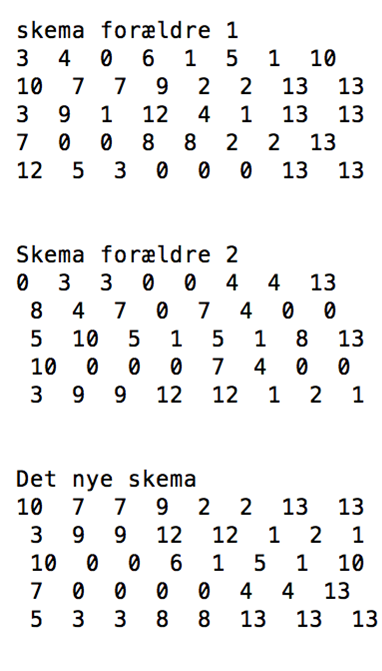
\includegraphics{partials/graphics/crossovertest.png}
  \caption{to parents og et child}
  \label{fig:crossovertest}
\end{figure}

Her er printet to parents skemaer for et child skema med dagene vandret og blokkene lodret. Her ses det at child skemaet har taget sin 1. dag fra første parents, sin 2. dag fra anden forældres sidste dag. 3. dag er første del af 4. dag fra anden forældre og sidste del af dag 1 fra første forældre. 4. dag foregår på samme måde og 5. dag er så de manglende lektioner der bliver indsat, indtil kravene er nået. Herefter bliver resten af lektionerne sat til at være 13 (fri).

